\documentclass[aspectratio=169]{beamer}
% -- Formato
% -- Paquetes base
\usepackage[utf8]{inputenc}
\usepackage[T1]{fontenc}
\usepackage[spanish]{babel}
\usepackage{booktabs}
\usepackage{iftex}
\usepackage{enumitem}
\usepackage{silence}
    \WarningsOff[beamerthememetropolis]

   
% -- Tipo de letra
\ifPDFTeX % LaTeX y pdfLaTeX
    \usepackage[defaultfam,tabular,lining]{montserrat}
        \renewcommand*\oldstylenums[1]{{\fontfamily{Montserrat-TOsF}\selectfont #1}}
    \usepackage[OT1]{eulervm}
    \renewcommand{\labelitemi}{$\bullet$}
    \DeclareMathSizes{10}{10.78}{7}{7}
\else % XeLaTeX
    \usepackage[OT1]{eulervm}
    \usepackage{fontspec}
    \setmainfont{montserrat}
    \DeclareSymbolFont{operators}{\encodingdefault}{\familydefault}{m}{n}
    \renewcommand{\labelitemi}{$\bullet$}
    \DeclareMathSizes{10}{10.78}{7}{7}
\fi 

% -- Espaciado
\addtolength{\abovedisplayskip}{-2.5mm}
\addtolength{\belowdisplayskip}{-2.5mm}
\setlength{\parskip}{0.3\baselineskip}

% -- Fondos
\newcommand{\fondo}[1]{
    % Selecciona el fondo
    \setbeamertemplate{background}{\includegraphics[width=\paperwidth]{Fondo/#1}}
    \ifthenelse{\equal{#1}{blanco}}{\setlength{\headsep}{42pt}}{\setlength{\headsep}{0pt}}
    }

% -- Formato 
\usetheme{metropolis}
\metroset{titleformat=smallcaps, numbering=fraction}
\usecolortheme{orchid}
    \definecolor{azul}{RGB}{19, 67, 131}
    \definecolor{gris}{RGB}{88, 88, 87}
    \definecolor{celeste}{RGB}{26, 160, 220}
    % -- Título en hoja de título
    \setbeamercolor{title}{fg=white}
    % -- Título de secciones
    \setbeamercolor{titlelike}{fg=white}
    % -- Texto
    \setbeamercolor{normal text}{fg=gris}
    % -- Título de diapositiva
    \setbeamercolor{frametitle}{fg=azul,bg=}
    % -- Color de fondo en bloques
    \setbeamercolor{block title}{fg=white,bg=azul}
    \setbeamercolor{block body}{bg=azul!15}
    \setbeamercolor{block title alerted}{fg=white,bg=celeste}
    \setbeamercolor{block body alerted}{bg=celeste!15}
    % -- Texto en hoja de título
    \setbeamercolor{author}{fg=celeste}
    \setbeamerfont{author}{series=\bfseries}
    \setbeamercolor{date}{fg=celeste}
    \setbeamerfont{date}{series=\bfseries}
    \setbeamercolor{institute}{fg=celeste}
    \setbeamerfont{institute}{series=\bfseries}
    % -- Barra de progreso
    \setbeamercolor{progress bar}{bg=white, fg=white}
    % -- Linea de separación en la página de título
    \makeatletter
    \setbeamertemplate{title separator}{
        \begin{tikzpicture}
            \fill[white] (0,0) rectangle (0.8\textwidth, \metropolis@titleseparator@linewidth);
        \end{tikzpicture}%
        \par%
    }
    \makeatother
    % -- Bloques redomdeados
    \setbeamertemplate{blocks}[rounded][shadow=true]
    % -- Caja de postit
    \setbeamercolor{postit}{fg=white,bg=celeste}
    \newenvironment{postitbox}[1][5cm]
        {~\begin{beamercolorbox}[sep=0.2em,wd=#1,rounded=true,shadow=true]{postit}}
        {\end{beamercolorbox}~}
    % -- Caja de postit para imagen
    \newcommand{\postitimg}[2][5cm]
        {
        ~\begin{beamercolorbox}[sep=0em,wd=#1,rounded=true,shadow=true]{postit}
        \includegraphics[width=\linewidth]{#2}
        \end{beamercolorbox}~
        }
    % -- Número de diapositiva
    \setbeamercolor{frame numbering}{fg=white}
    \setbeamerfont{page number in head/foot}{size=\tiny}
    \setbeamertemplate{footline}{
        \begin{beamercolorbox}[wd=\textwidth, center, sep=16.5mm]{footline}%
            \usebeamerfont{page number in head/foot}%
            \usebeamertemplate*{frame numbering}
        \end{beamercolorbox}%
    }
    % -- Tabla de contenidos
    \makeatletter
    \patchcmd{\beamer@sectionintoc}
      {\vfill}
      {\vskip\itemsep}
      {}
      {}
    \makeatother  
    \setbeamertemplate{section in toc}{%
    \inserttocsectionnumber.  \inserttocsection \par}
    % -- Agregar margen superior
    \addtolength{\headsep}{14mm}
    \addtobeamertemplate{frametitle}{\vspace*{-2mm}}{\vspace*{-3mm}}

 % -- Formato de bibliografía
\usepackage{csquotes}
\usepackage[backend=biber, style=apa]{biblatex}
% -- Adaptar apa al español (2023)
    \makeatletter
    \DefineBibliographyExtras{spanish}{ 
        % Código para corregir &
        \setcounter{smartand}{1}
    	\let\lbx@finalnamedelim=\lbx@es@smartand
    	\let\lbx@finallistdelim=\lbx@es@smartand
        % Código para corregir coma final
        \renewcommand*{\apablx@ifrevnameappcomma}[2]{#2}
        \let\finalandcomma=\empty
    }
    \makeatother
    \setlength{\bibhang}{\parindent}
% -- Fin de adaptar apa al español (2023)   
    



% -- Paquetes adicionales
\usepackage{aleph-comandos}

% -- Comandos extra


% -- Datos
\title{Ciencia de Datos para el reconocimiento de imágenes}
% \subtitle{}
\author{Mat. Andrés Merino, MSc}
\institute{Carrera de Ciencia de Datos}
\date{Junio - 2024}

%%%%%%%%%%%%%%%%%%%%%%%%%%%%%%%%%%%%%%%%
\begin{document}

%%%%%%%%%%%%%%%%%%%%%%%%%%%%%%%%%%%%%%%%
%% Página de título
\fondo{inicio}
\begin{frame}[plain]
\addtocounter{framenumber}{-1}
    \titlepage
\end{frame}

% %%%%%%%%%%%%%%%%%%%%%%%%%%%%%%%%%%%%%%%%
% %% Página de índice 
% \fondo{blanco}
% \begin{frame}[plain]
%     \titulo{Contendio}
    
%     \tableofcontents
% \end{frame}

%%%%%%%%%%%%%%%%%%%%%%%%%%%%%%%%%%%%%%%%
%% Sección 1
%%%%%%%%%%%%%%%%%%%%%%%%%%%%%%%%%%%%%%%%%%%%%%%%%%%%%%%%
\fondo{celeste}
\section{Motivación}
\fondo{blanco}
%%%%%%%%%%%%%%%%%%%%%%%%%%%%%%%%%%%%%%%%%%%%%%%%%%%%%%%%


%%%%%%%%%%%%%%%%%%%%%%%%%%%%%%%%%%%%%%%%%%%%%%%%%%%%%%%%
%%%%%%%%%%%%%%%%%%%%%%%%%%%%%%%%%%%%%%%%%%%%%%%%%%%%%%%%
\begin{frame}{¿Qué hay en esta foto?}

    \begin{center}
        \postitimg[5.5cm]{Figuras/Fig01.jpg}
    \end{center}

\end{frame}


%%%%%%%%%%%%%%%%%%%%%%%%%%%%%%%%%%%%%%%%%%%%%%%%%%%%%%%%
%%%%%%%%%%%%%%%%%%%%%%%%%%%%%%%%%%%%%%%%%%%%%%%%%%%%%%%%
\begin{frame}
    \begin{columns}
    \column{6cm}
        \postitimg[5.5cm]{Figuras/Fig02.jpg}\pause
    \column{6cm}
        \postitimg[4.5cm]{Figuras/Fig03.jpg}
    \end{columns}

\end{frame}


%%%%%%%%%%%%%%%%%%%%%%%%%%%%%%%%%%%%%%%%%%%%%%%%%%%%%%%%
%%%%%%%%%%%%%%%%%%%%%%%%%%%%%%%%%%%%%%%%%%%%%%%%%%%%%%%%
% \begin{frame}

%     \begin{columns}
%     \column{7.5cm}
%         \postitimg[7cm]{Figuras/Fig04.png}
%         \\[1.5cm]\hspace{0pt}
%         \pause
%     \column{7.5cm}
%         \hspace{0pt}\\[2cm]
%         \postitimg[7cm]{Figuras/Fig05.png}
%     \end{columns}

% \end{frame}

%% Sección 2
%%%%%%%%%%%%%%%%%%%%%%%%%%%%%%%%%%%%%%%%%%%%%%%%%%%%%%%%
\fondo{celeste}
\section{Matrices}
\fondo{blanco}
%%%%%%%%%%%%%%%%%%%%%%%%%%%%%%%%%%%%%%%%%%%%%%%%%%%%%%%%


%%%%%%%%%%%%%%%%%%%%%%%%%%%%%%%%%%%%%%%%%%%%%%%%%%%%%%%%
%%%%%%%%%%%%%%%%%%%%%%%%%%%%%%%%%%%%%%%%%%%%%%%%%%%%%%%%
\begin{frame}

    \begin{block}{Matrices}
        Una matriz es un arreglo de números de la forma:
        \[
            A = 
            \begin{pmatrix}
            a_{0,0} & a_{0,1} & \cdots & a_{0,n-1} \\ 
            a_{1,0} & a_{1,1} & \cdots & a_{1,n-1} \\ 
            \vdots & \vdots & \ddots & \vdots\\ 
            a_{m-1,0} & a_{m-1,1} & \cdots & a_{m-1,n-1}
            \end{pmatrix}.
        \]
        Con esto, se dice que $A$ es de orden $m \times n$ y que tiene $m$ filas y $n$ columnas. Al conjunto de todas las matrices de orden $m \times n$ se denota por $\Mat[\R]{m}{n}$.
    \end{block}

\end{frame}


%%%%%%%%%%%%%%%%%%%%%%%%%%%%%%%%%%%%%%%%%%%%%%%%%%%%%%%%
%%%%%%%%%%%%%%%%%%%%%%%%%%%%%%%%%%%%%%%%%%%%%%%%%%%%%%%%
\begin{frame}{Ejemplos}

\end{frame}


%%%%%%%%%%%%%%%%%%%%%%%%%%%%%%%%%%%%%%%%%%%%%%%%%%%%%%%%
%%%%%%%%%%%%%%%%%%%%%%%%%%%%%%%%%%%%%%%%%%%%%%%%%%%%%%%%
% \begin{frame}[fragile]

%     \titulo{¿Puedo hacer esto en la compu?}

% \begin{pycodigo}
% \begin{ipynbcodigo}
% \begin{lstlisting}[language=Python]
% from numpy import np
% \end{lstlisting}
% \end{ipynbcodigo}
% \begin{ipynbcodigo}
% \begin{lstlisting}[language=Python]
% A = np.array([
%     [1, 0, 1],
%     [0, 1, 0]
%     ])
% print(A)
% \end{lstlisting}
% \end{ipynbcodigo}
% \end{pycodigo}

% \end{frame}


%%%%%%%%%%%%%%%%%%%%%%%%%%%%%%%%%%%%%%%%%%%%%%%%%%%%%%%%
%%%%%%%%%%%%%%%%%%%%%%%%%%%%%%%%%%%%%%%%%%%%%%%%%%%%%%%%
\begin{frame}

    \begin{block}{Suma de matrices}
        Dadas dos matrices $A$ y $B$ del mismo orden, se define la suma de matrices, $A+B$, a la matriz que resulta de sumar, componente a componete, las componentes de las matrices.
    \end{block}
    \vspace{3cm}

\end{frame}

% %%%%%%%%%%%%%%%%%%%%%%%%%%%%%%%%%%%%%%%%%%%%%%%%%%%%%%%%
% %%%%%%%%%%%%%%%%%%%%%%%%%%%%%%%%%%%%%%%%%%%%%%%%%%%%%%%%
% \begin{frame}

%     \begin{block}{Multiplicación de matrices por un escalar}
%         Dada una matriz $A$ y un número real $\alpha$, se define la multiplicación de una matriz por un escalar, $\alpha A$, a la matriz que resulta de multiplicar, cada componete, por el número $\alpha$.
%     \end{block}
%     \vspace{3cm}

% \end{frame}
%% Sección 3
%%%%%%%%%%%%%%%%%%%%%%%%%%%%%%%%%%%%%%%%%%%%%%%%%%%%%%%%
\fondo{celeste}
\section{¿Qué es una imagen?}
\fondo{blanco}
%%%%%%%%%%%%%%%%%%%%%%%%%%%%%%%%%%%%%%%%%%%%%%%%%%%%%%%%


%%%%%%%%%%%%%%%%%%%%%%%%%%%%%%%%%%%%%%%%%%%%%%%%%%%%%%%%
%%%%%%%%%%%%%%%%%%%%%%%%%%%%%%%%%%%%%%%%%%%%%%%%%%%%%%%%
\begin{frame}{¿Que es una imagen?}

    \vspace{1cm}
    \begin{columns}
    \column{6cm}
        Consideremos esta matriz
        \[
            img = \begin{pmatrix}
                1& 0& 1& 0\\
                0& 1& 0& 1
            \end{pmatrix}.
        \]
        ¿Qué pasa si donde hay un 1 lo pinto de blanco y donde hay un 0 lo pinto de negro?\pause
    \column{6cm}
        \postitimg[6cm]{Figuras/Fig06}
    \end{columns}

\end{frame}


%%%%%%%%%%%%%%%%%%%%%%%%%%%%%%%%%%%%%%%%%%%%%%%%%%%%%%%%
%%%%%%%%%%%%%%%%%%%%%%%%%%%%%%%%%%%%%%%%%%%%%%%%%%%%%%%%
\begin{frame}{Ejemplo}
    
    \vspace{0.5cm}
    Prueba con la matriz
    \[
        img1 = \begin{pmatrix}
            1& 0& 1& 0& 1\\
            0& 1& 0& 1& 0\\
            0& 1& 1& 1& 0\\
            1& 0& 1& 0& 1\\
            1& 1& 0& 1& 1\\
        \end{pmatrix}
    \]
    \vfill

\end{frame}

%%%%%%%%%%%%%%%%%%%%%%%%%%%%%%%%%%%%%%%%%%%%%%%%%%%%%%%%
%%%%%%%%%%%%%%%%%%%%%%%%%%%%%%%%%%%%%%%%%%%%%%%%%%%%%%%%
\begin{frame}{Ejemplo}
    
    \vspace{0.5cm}
    Prueba con la matriz
    \[
        img2 = \begin{pmatrix}
            1& 1  & 1  & 1  & 1\\
            1& 0.5& 0  & 0.5& 1\\
            1& 0.5& 0.5& 0.5& 1\\
            1& 1  & 0.5& 1  & 1\\
            1& 1  & 1  & 1  & 1\\
        \end{pmatrix}
    \]
    \vfill

\end{frame}

%%%%%%%%%%%%%%%%%%%%%%%%%%%%%%%%%%%%%%%%%%%%%%%%%%%%%%%%
%%%%%%%%%%%%%%%%%%%%%%%%%%%%%%%%%%%%%%%%%%%%%%%%%%%%%%%%
\begin{frame}{Ejemplo}
    
    \vspace{0.5cm}
    Prueba con la matriz
    \[
        img1 + img2
    \]
    \vfill

\end{frame}

%%%%%%%%%%%%%%%%%%%%%%%%%%%%%%%%%%%%%%%%%%%%%%%%%%%%%%%%
%%%%%%%%%%%%%%%%%%%%%%%%%%%%%%%%%%%%%%%%%%%%%%%%%%%%%%%%
\begin{frame}

    \hspace*{-.5cm}
    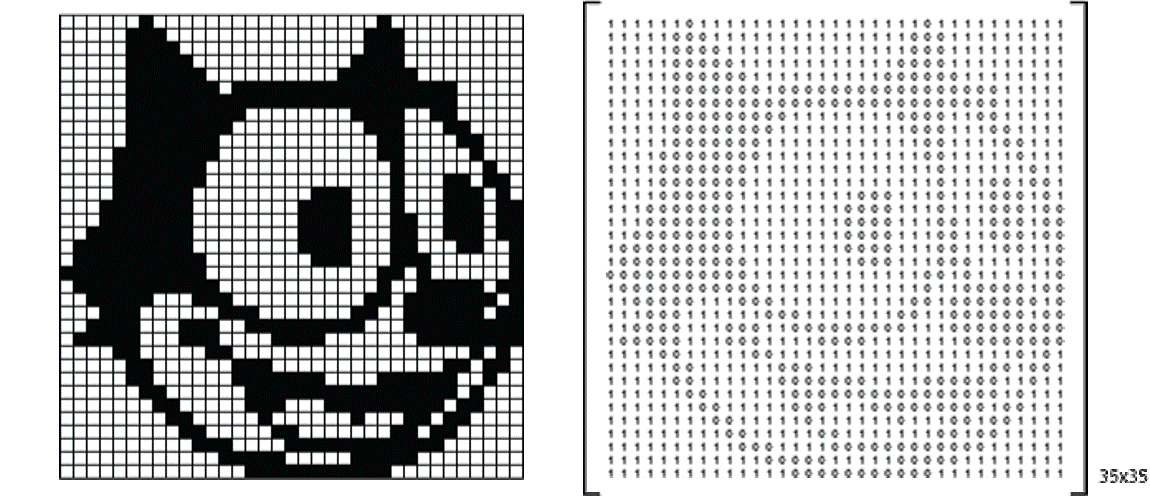
\includegraphics[width=15cm]{Figuras/Fig07}

\end{frame}
%% Sección 4
%%%%%%%%%%%%%%%%%%%%%%%%%%%%%%%%%%%%%%%%%%%%%%%%%%%%%%%%
\fondo{celeste}
\section{Imágenes a color}
\fondo{blanco}
%%%%%%%%%%%%%%%%%%%%%%%%%%%%%%%%%%%%%%%%%%%%%%%%%%%%%%%%


%%%%%%%%%%%%%%%%%%%%%%%%%%%%%%%%%%%%%%%%%%%%%%%%%%%%%%%%
%%%%%%%%%%%%%%%%%%%%%%%%%%%%%%%%%%%%%%%%%%%%%%%%%%%%%%%%
\begin{frame}{El formato RGB}

    \begin{columns}
    \column{8cm}
        Es un modelo de color basado en la síntesis aditiva, con el que es posible representar un color mediante la mezcla por adición de los tres colores de luz primarios: \textcolor{red}{rojo}, \textcolor{green}{verde} o \textcolor{blue}{azul}
    \column{5cm}
        \postitimg[5cm]{Figuras/Fig08}
    \end{columns}

\end{frame}


%%%%%%%%%%%%%%%%%%%%%%%%%%%%%%%%%%%%%%%%%%%%%%%%%%%%%%%%
%%%%%%%%%%%%%%%%%%%%%%%%%%%%%%%%%%%%%%%%%%%%%%%%%%%%%%%%
\begin{frame}{Ejemplo}
    \[
        R = \begin{pmatrix}
            0.0& 0.3& 0.9\\
            1.0& 0.0& 1.0
        \end{pmatrix};\quad
        G = \begin{pmatrix}
            0.0& 0.3& 0.3\\
            0.0& 1.0& 1.0
        \end{pmatrix};\quad
        B = \begin{pmatrix}
            0.0& 0.3& 0.9\\
            0.0& 0.0& 1.0
        \end{pmatrix}.
    \]
    \pause  
    \begin{center}
    \postitimg[4cm]{Figuras/Fig09}
    \end{center}

\end{frame}

%%%%%%%%%%%%%%%%%%%%%%%%%%%%%%%%%%%%%%%%%%%%%%%%%%%%%%%%
%%%%%%%%%%%%%%%%%%%%%%%%%%%%%%%%%%%%%%%%%%%%%%%%%%%%%%%%
\begin{frame}{Jueguemos con Mario}
    
    \begin{center}
    \postitimg[3.5cm]{Figuras/Mario}
    \end{center}

\end{frame}

%% Sección 5
%%%%%%%%%%%%%%%%%%%%%%%%%%%%%%%%%%%%%%%%%%%%%%%%%%%%%%%%
\fondo{celeste}
\section{Filtros}
\fondo{blanco}
%%%%%%%%%%%%%%%%%%%%%%%%%%%%%%%%%%%%%%%%%%%%%%%%%%%%%%%%


%%%%%%%%%%%%%%%%%%%%%%%%%%%%%%%%%%%%%%%%%%%%%%%%%%%%%%%%
%%%%%%%%%%%%%%%%%%%%%%%%%%%%%%%%%%%%%%%%%%%%%%%%%%%%%%%%
\begin{frame}{Filtros}

    \vspace*{-2.5cm}
    \begin{columns}
    \column{3cm}
        
        \href{https://mlnotebook.github.io/img/CNN/convSobel.gif}{Ver animación.}
    \column{8cm}
    \begin{center}
        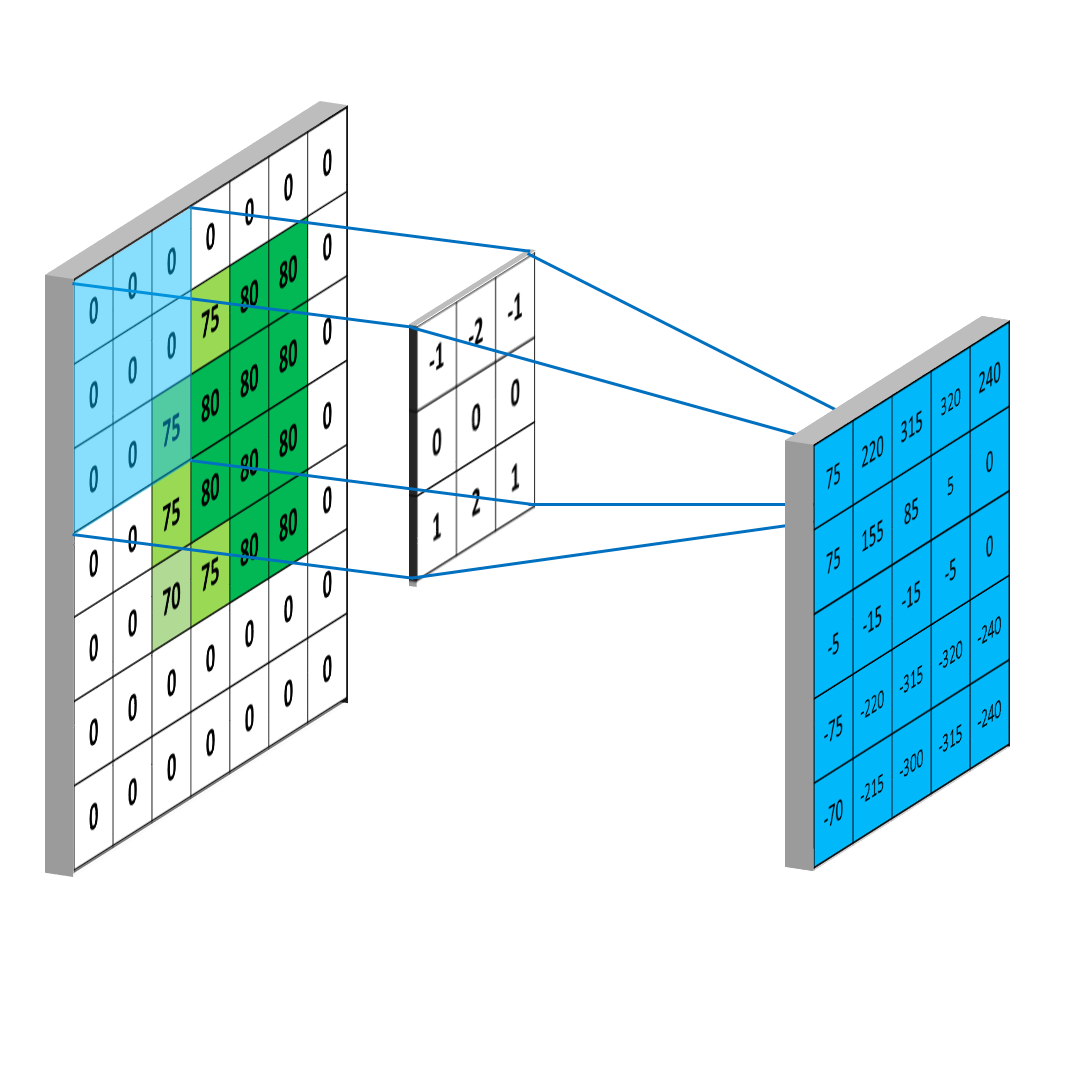
\includegraphics[height=9.5cm]{Figuras/Fig10}
    \end{center}
    \end{columns}
    
\end{frame}

%%%%%%%%%%%%%%%%%%%%%%%%%%%%%%%%%%%%%%%%%%%%%%%%%%%%%%%%
%%%%%%%%%%%%%%%%%%%%%%%%%%%%%%%%%%%%%%%%%%%%%%%%%%%%%%%%
\begin{frame}{Jueguemos con Bowser}
    
    \begin{center}
    \postitimg[8.5cm]{Figuras/Bowser}
    \end{center}

\end{frame}



%%%%%%%%%%%%%%%%%%%%%%%%%%%%%%%%%%%%%%%%%%%%%%%%%%%%%%%%
%%%%%%%%%%%%%%%%%%%%%%%%%%%%%%%%%%%%%%%%%%%%%%%%%%%%%%%%
\begin{frame}{Prueba los siguientes filtros}
    \[
        \begin{pmatrix}
            -2& -1& 0\\
            -1& 1& 1\\
             0& 1& 2
        \end{pmatrix};\quad
        \begin{pmatrix}
            -1& -1& -1\\
            0& 0& 0\\
            1& 1& 1
        \end{pmatrix};\quad
        \begin{pmatrix}
            1& 0& -1\\
            1& 0& -1\\
            1& 0& -1
        \end{pmatrix}.
    \]

\end{frame}


%%%%%%%%%%%%%%%%%%%%%%%%%%%%%%%%%%%%%%%%%%%%%%%%%%%%%%%%
\fondo{celeste}
\section{Reconocimiento de imágenes}
\fondo{blanco}
%%%%%%%%%%%%%%%%%%%%%%%%%%%%%%%%%%%%%%%%%%%%%%%%%%%%%%%%

%%%%%%%%%%%%%%%%%%%%%%%%%%%%%%%%%%%%%%%%%%%%%%%%%%%%%%%%
%%%%%%%%%%%%%%%%%%%%%%%%%%%%%%%%%%%%%%%%%%%%%%%%%%%%%%%%
\begin{frame}{¿Qué hay en esta foto?}
    
    \begin{center}
    \postitimg[7cm]{Figuras/OsoAurelio}
    \end{center}

\end{frame}


% %%%%%%%%%%%%%%%%%%%%%%%%%%%%%%%%%%%%%%%%
% %% Página de referencias
% \begin{frame}[allowframebreaks]    
%     \titulo{Bibliografía}
%     \bibliographystyle{apalike}
%     \nocite{*}
%     \bibliography{referencias.bib}
% \end{frame}

%%%%%%%%%%%%%%%%%%%%%%%%%%%%%%%%%%%%%%%%
%% Página final
\fondo{final}
\begin{frame}[plain]
\begin{center}
    \color{white}
    {\Huge\textbf{¡Estudia Ciencia de Datos!}}

    \vspace{1cm}
    \textcolor{azul}{\textbf{Contacto:}} aemerinot@puce.edu.ec
\end{center}
\end{frame}


\end{document}